% Appendix A

\chapter{Physical models} % Main appendix title

\label{AppendixA} % For referencing this appendix elsewhere, use \ref{AppendixA}

\lhead{Appendix A. \emph{Physical models}} % This is for the header on each page - perhaps a shortened title

In IM3D code, the simulation of ion transportation in matter proceeds is similar to the well-established TRIM-like codes, which basically introduces the random phase approximation (RPA), the binary collision approximation (BCA) and the central potential approximation (CPA)\cite{Ziegler:2010,Schiettekatte:2008,Biersack:1980}. The code simulates numerical random trajectory histories of ions to present statistically meaningful calculation results. Each trajectory corresponds to a particle (ion or target atom) with a specified starting position, a given direction and an incident energy. The particle is tracked as a random sequence of straight free-flight-paths that end with a binary nuclear collision event where the particle changes its direction of movement and/or reduces energy as a result of nuclear (elastic collision process) and electronic (inelastic collision process) energy losses. The energy and direction of the particle from incident direction are thus updated from the conservation of energy and momentum. Where, the probability of energy losses depends on the target atom density, as well as the nuclear and electronic stopping powers which can be assumed to be independent. Meanwhile, point defects could be produced in elastic collision events. Finally, the trajectory is terminated till the energy of the particle drops below a specified value $E_{min}$ or the particle leaves the target. A program chart of the ions tracing and defects generation in a target is given in Fig.\ref{Fig.1} and the detailed physical background can also be found elsewhere\cite{Ziegler:2010}.

\begin{figure}[!ht]\centering
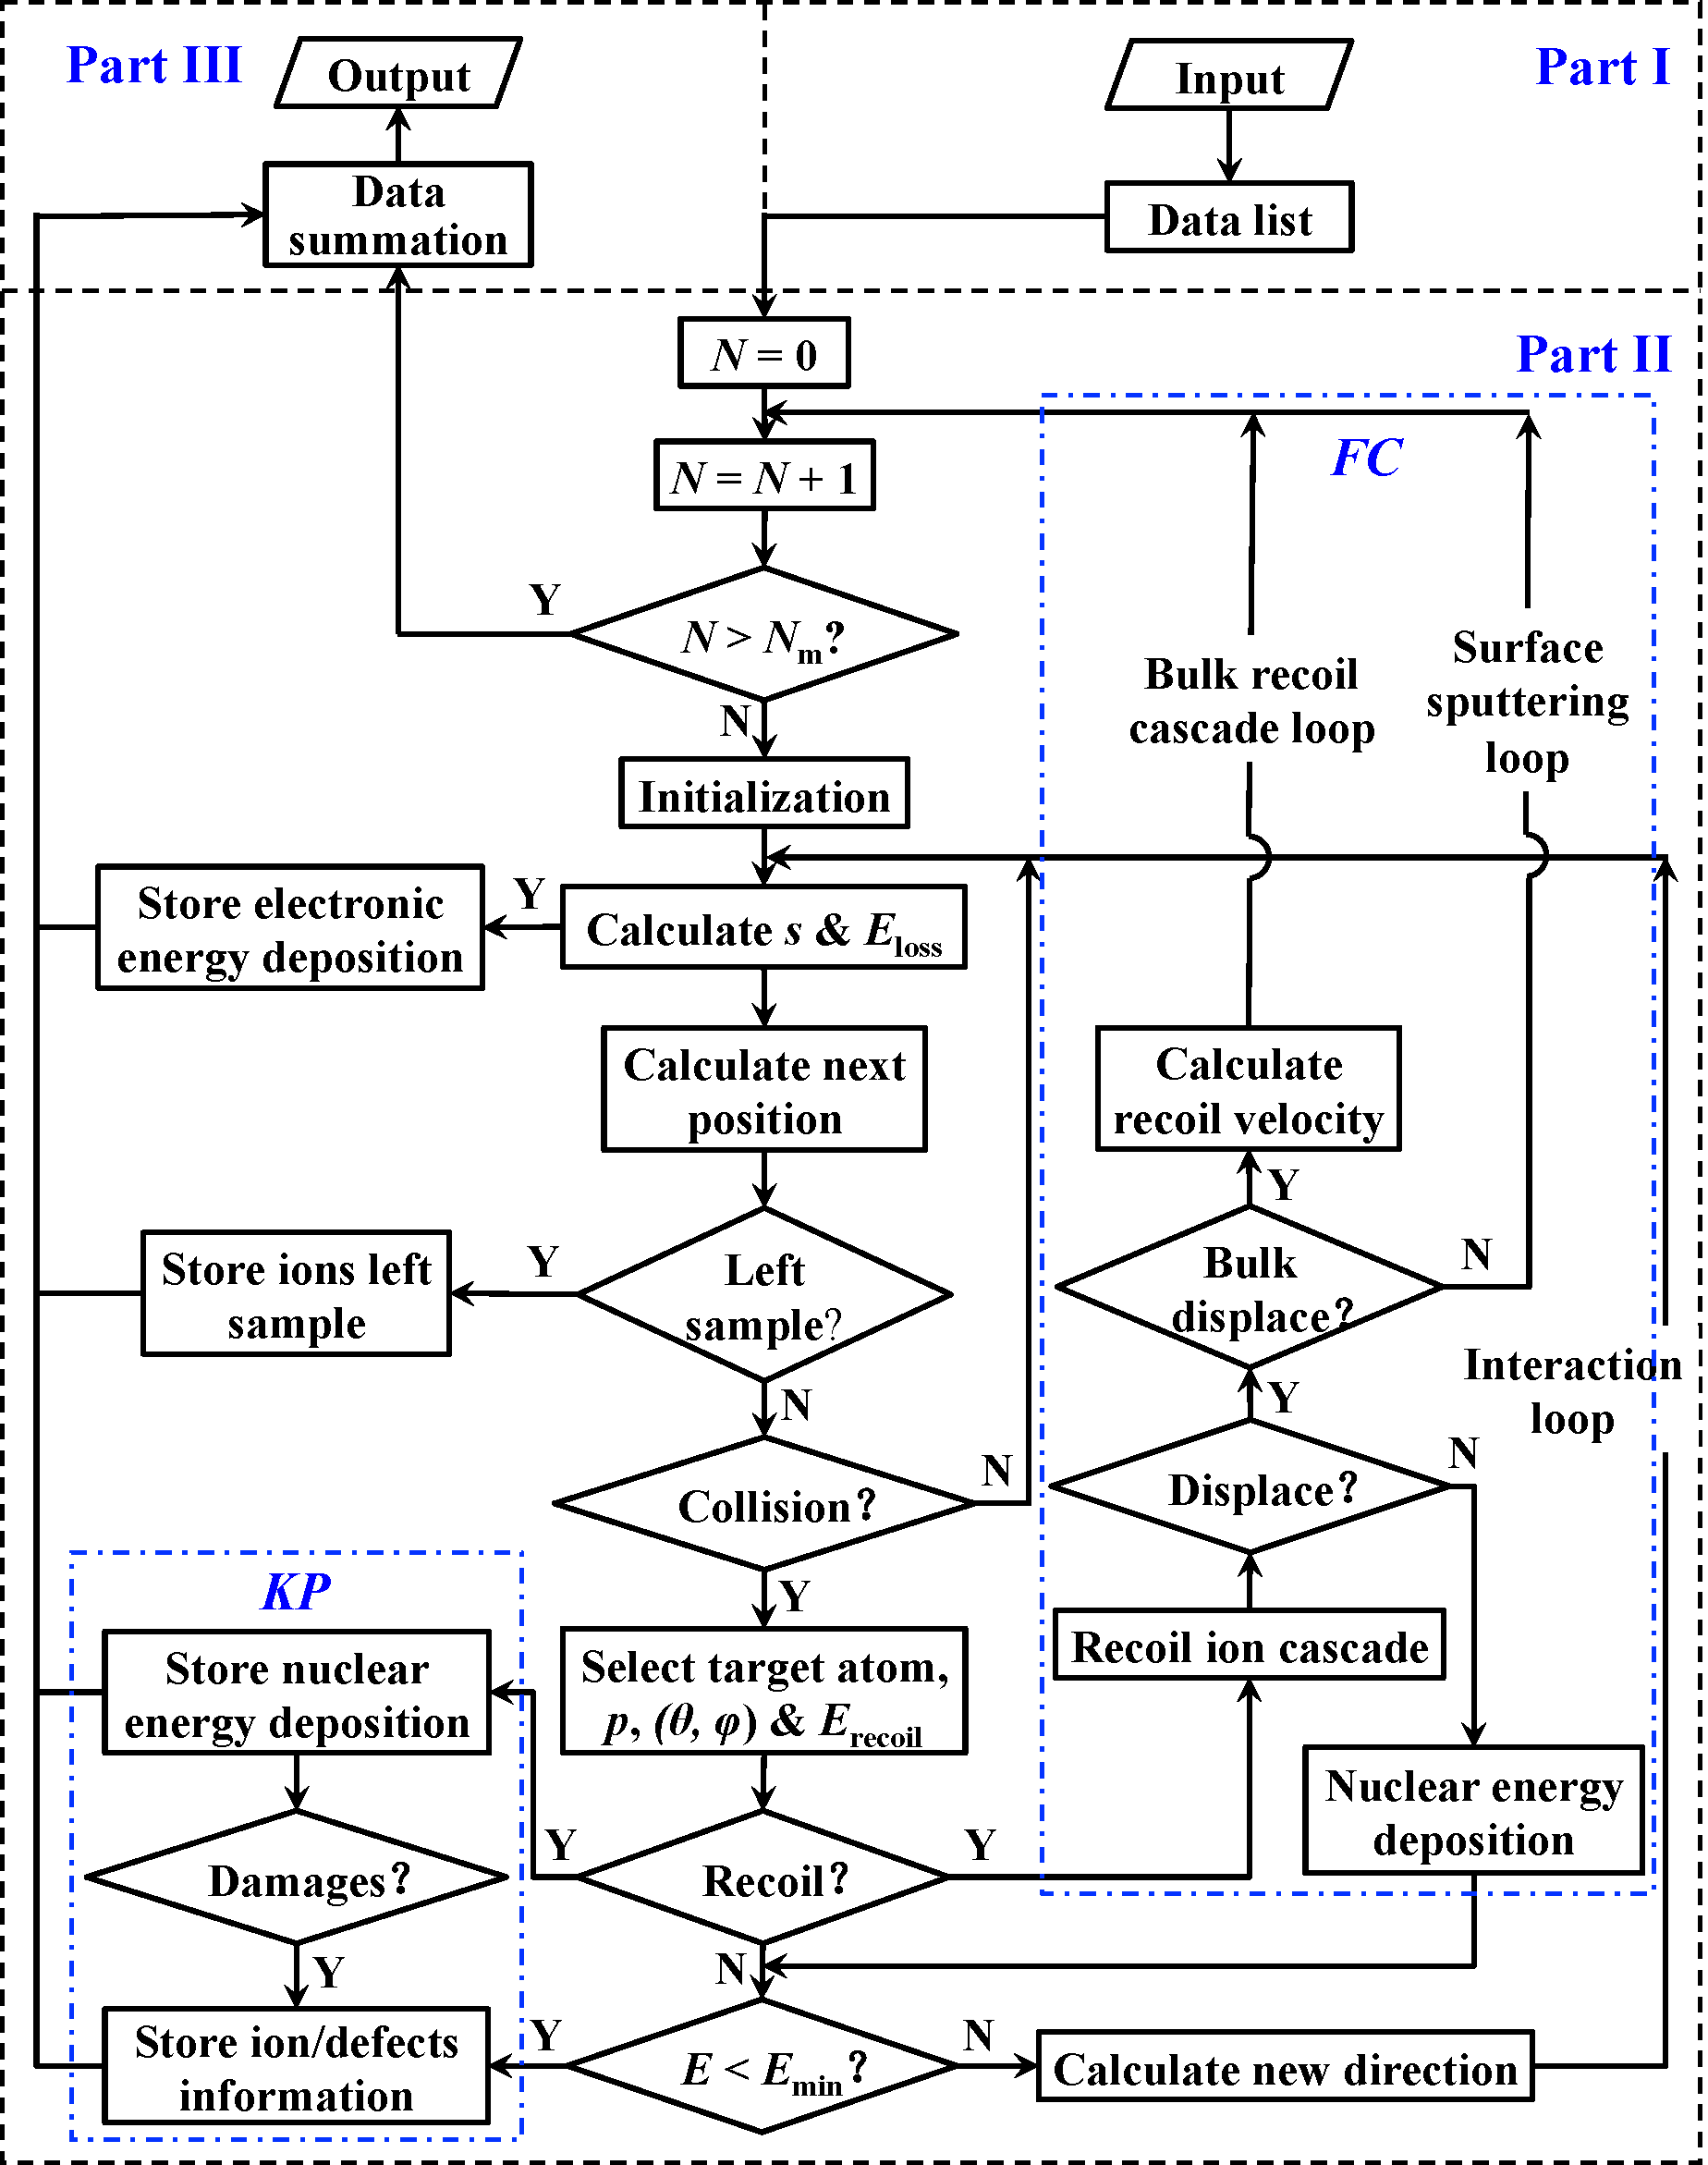
\includegraphics[width=0.68\textwidth]{fig1.pdf}
\caption{IM3D program chart of ions tracing and defects generation in a sample.} \label{Fig.1}
\end{figure}

For the elastic collision process, the classical binary atomic scattering angle $\theta_{CM}$ in the center-of-mass (CM) coordinate system can be evaluate accurately from the famous ``scattering integral" as,
\begin{equation}
\theta_{CM} = \pi - 2 \int_{r_0}^{\infty} \frac{p \cdot dr}{r^2 \sqrt{1 - \frac{V \left( r \right)}{E_c} - \left( \frac{p}{r} \right)^2}} \label{Eq.0}
\end{equation}
\noindent where, $p$ is the impact parameter, $r_0$ is the closet distance ($r$) between two atoms during the collision, $V\left( r \right)$ is the screened inter-atomic potential as listed below and $E_c$ is the kinetic energy of the incident atom in the center-of-mass frame. This integral can not be calculated analytically for inter-atomic screening potentials and hence a time-consuming numerical integration must be used instead\cite{Ziegler:2010}. An analytical approximation formula (such as the MAGIC approximation\cite{Ziegler:2010}) or a lookup table method (such as the fast indexing technique\cite{Schiettekatte:2008}) can be used in terms of accuracy and efficiency, as described in Section 2.3. The interaction potential $V \left( r \right)$ between two atoms is a screened repulsive Coulomb potential described by a dimensionless screening function, such as the Thomas-Feimi potential\cite{Sommerfeld:1932}, the Lenz-Jensen potential\cite{Lenz:1932}, the Moliere potential\cite{Moliere:1947}, the Bohr potential\cite{Bohr:1948} and the universal Ziggler-Biersack-Littmark (ZBL) potential\cite{Ziegler:2010}. In addition, the recoil energy of a target atom due to elastic nuclear collisions can be evaluated by the BCA between two charged particles involved in one scattering process.

For the inelastic collision process, the ion energy reduce uniformly along the free-flight-paths though the electronic energy losses accounting for the energy straggling. In IM3D code, the physical parameters such as electronic energy stopping powers are generated from SRModule.exe provided by SRIM package\cite{Ziegler:2004}, in the form of pre-calculated tables as implemented in Corteo\cite{Schiettekatte:2008}.
%In SRIM package (?), the Lindhard-Scharff formula for low energies and the Bethe-Bloch formula for high energies are used for evaluating electronic stopping cross sections, while the interpolation scheme is applied to provide a realistically smooth transition to bridge the gap between the low and high energy regions\cite{Biersack:1980}.
Either Bohr\cite{Bohr2:1948}, Chu\cite{Chu:1976} or Wang\cite{Yang:1991} formula can be selected to considering the energy straggling. Furthermore, IM3D code also employ a linear addition of stopping powers (known as Bragg's rule\cite{Bragg:1905}) for determining the stopping power in alloys, compounds and mixtures.

The generation of point defects (i.e. interstitials and vacancies) can be modeled by the analytical modified Kinchin-Pease (KP) model\cite{Kinchin:1955,Norgett:1975} or the computationally full cascade (FC) simulation.
%The modified KP model can only estimate the number of vacancies and assume the same local concentration for interstitials produced in a collision cascade, while the FC simulation can accurately determine the location of the interstitials by tracing the trajectories of all recoiling atoms in a collision cascade but requires a greater computational effort.
%By comparing to NRT and MD calculation results, Stroller et. al pointed out that it is recommended that when direct comparisons between ion and neutron data are intended, the KP option of SRIM code should be selected\cite{Stoller:2013}.
Assume a trajectory atom with atomic number $Z_1$ and energy $E$ collide with a target atom with atomic number $Z_2$. After the collision event, the energy of the trajectory atom change to $E_1$ and the target atom obtains energy $E_2$, and thus different damage generation processes would also occur: (1) if $E_2 > E_d$ ($E_d$ is the displacement energy of the target atom), a displacement occurs so that the target atom has enough energy to leave the site; (2) if both $E_1 > E_d$ and $E_2 > E_d$, a vacancy occurs; (3) if $E_2 < E_d$, the target atom without enough energy will vibrate back to its site releasing energy $E_2$ as phonons; (4) if $E_1 < E_b$ ($E_b$ is the lattice/surface binding energy of the target atom), $E_2 > E_d$ and $Z_1 = Z_2$, a replacement collision occurs with energy $E_1$ releasing as phonons; (5) if ($E_1 < E_{min}~or~E_b$, $E_2 > E_d$ and $Z_1 \neq Z_2$) or ($E_1 < E_{min}~or~E_b$ and $E_2 < E_d$), the trajectory atom becomes an interstitial atom.
